\documentclass[12pt]{article}

\usepackage{sbc-template}
\usepackage{booktabs}
\usepackage{graphicx,url}
\usepackage{hyperref}
%\usepackage[brazil]{babel}
\usepackage[utf8]{inputenc}
\usepackage[brazil]{babel}
\usepackage{booktabs}
\usepackage{amsmath}

%% Comandos para comentários -- elloa
\usepackage{xcolor}
\definecolor{lightblue}{RGB}{0,191,255}
\usepackage[textsize=tiny,backgroundcolor=lightblue,linecolor=lightblue]{todonotes}
%%%%%% Subfiguras -- elloa
\usepackage[bf,sf,footnotesize,indent,justification=centering]{caption}
\usepackage[caption=true,font=footnotesize]{subfig}
\captionsetup[subfigure]{justification=centering,labelfont={bf,sf},textfont={bf,sf,footnotesize},singlelinecheck=off,justification=centering}
\captionsetup[figure]{justification=centering,labelfont={bf,sf},textfont={bf,sf,footnotesize},singlelinecheck=off}
\captionsetup[table]{justification=centering,labelfont={bf,sf},textfont={bf,sf,footnotesize},singlelinecheck=off,justification=centering}
%%%%%%%%%%%%%%%%%%%%%%%%%%%%%%%%%%%%%%%%%%

\sloppy

\title{Classificação de Expressões Faciais com \emph{Ensemble} de Redes Neurais Convolucionais e Votação Inteligente}

\author{Rodrigo C. Moraes, Carlos Maurício S. Figueiredo, Elloá B. Guedes}


\address{Núcleo de Computação\\
Escola Superior de Tecnologia\\
Universidade do Estado do Amazonas\\
Av. Darcy Vargas, 1200 -- Manaus -- Amazonas
\email{\{rcm.eng, cfigueiredo, ebgcosta\}@uea.edu.br}}

\begin{document}

\maketitle

\begin{abstract}
Facial Expression is a very important factor in the social interaction of human beings. And technologies that can automatically interpret and respond to stimuli of facial expressions already find a wide variety of applications, from antidepressant drug testing to fatigue analysis of drivers and pilots. In this context, the following work presents a model for Automatic Classification of Facial Expression using as a training base the dataset Challenges in Representation Learning (FER2013), characterized by examples of spontaneous facial expressions in uncontrolled environments. The presented method is composed by a Convolutional Neural Networks Ensemble architecture, using a non-trivial voting system, based on a smart model, Xtreme Gradient Boosting - XGBoost. As performance criteria for validation of the proposed model, were used K-fold and F1 Score Micro techniques to guarantee robustness and reliability of the results, which are competitive with state-of-the-art works.
\end{abstract}

\begin{resumo}

A Expressão Facial é um fator de suma importância na interação social dos seres humanos. E tecnologias que podem interpretar e responder de forma automática a estímulos de expressões faciais já encontram uma grande variedade de aplicações, desde teste de fármacos antidepressivos, até análise de fadiga de motoristas e pilotos. Neste contexto, o seguinte trabalho apresenta um modelo para Classificação Automática de Expressão Facial utilizando como base de treinamento o \textit{dataset} \textit{Challenges in Representation Learning: Facial Expression Recognition Challenge}(FER2013), caracterizado por exemplos de expressões faciais espontâneas em ambientes não controlados.  O método apresentado é composto por uma arquitetura \textit{Ensemble} de Redes Convolucionais Neurais, utilizando um sistema de votação não-trivial, baseado em um modelo inteligente, \textit{Xtreme Gradient Boosting} - \textit{XGBoost}. Como critérios de desempenho para validação do modelo proposto foram empregadas técnicas de K-fold e F1 Score Micro, para garantia de robustez e confiança dos resultados, que são competitivos com trabalhos estado-da-arte.

\end{resumo}


\section{Introdução}
%https://ibug.doc.ic.ac.uk/media/uploads/documents/EncycBiometrics-Pantic-FacExpRec-PROOF.pdf
A Classificação de Expressões Faciais é um processo executado por humanos e computadores que consiste em localizar faces em uma cena, extrair características faciais da região detectada, analisar alterações das características faciais como um sorriso ou um franzir de sobracelhas, e categorizar o resultado em uma expressão como felicidade ou raiva, por exemplo \cite{Pantic2009fea}.

Tecnologias que podem interpretar e responder de forma automática a expressões faciais já encontram uma grande variedade de aplicações, dada sua importância social. Exemplos disto, são sistemas de ensino que utilizam a expressão facial dos alunos como \textit{feedback}, teste da efetividade de fármacos anti-depressivos e detecção de fadiga de motoristas e pilotos \cite{Fasel2003}.

Graças a introdução de métodos de \textit{Machine Learning}, tem-se  avançado no campo de Classificação Automática de Expressões Faciais. Mais especificamente, métodos de \textit{Deep Learning} tem apresentado resultados bons nas tarefas que envolvem o uso de detecção de padrões e extração de características em imagens, nas mais variadas situações e contextos \cite{whitehill2013automatic}.

Paul Ekman e Friesen postularão seis emoções primárias que possuem cada uma conteúdo próprio e associação a uma única expressão facial. Estas emoções se monstram invariantes ao longo das diversas culturas humanas e são identificadas como felicidade, tristeza, medo, nojo, surpresa e raiva \cite{Ekman1971}.

O presente trabalho apresentou resultados equiparáveis ao da literatura na tarefa de Classificação Automática de Expressões Faciais nas expressões primárias, utilizando modificação não-trivial, votação mediada por um modelo inteligente, em \textit{Emsemble} de Redes Neurais Convolucionais.


\section{Trabalhos Relacionados}
Relatar aqui os trabalhos análogos.


\section{Materiais e Métodos}
\subsection{Dados Experimentais}
A base de dados de expressões faciais utilizada para o desenvolvimento deste trabalho é denominada \emph{Facial Expression Recognition Challenge} (FER2013). Esta base contém $35.887$ imagens faciais em escala de cinza com dimensões de $48\times 48$ pixels, rotuladas de maneira supervisionada segundo uma das sete expressões faciais universais, conforme amostras ilustradas na Figura \ref{fig:samples}.

\begin{figure}[h!]
	\centering
  \captionof{figure}{Amostras de imagens faciais da base de dados FER2013.}
  \label{fig:samples}

	\begin{tabular}{@{}c@{}}
		\subfloat[Felicidade]{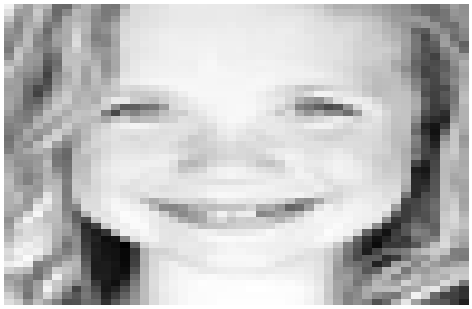
\includegraphics[width=0.15\linewidth]{images/sample_happy.png}}
		\subfloat[Nojo]{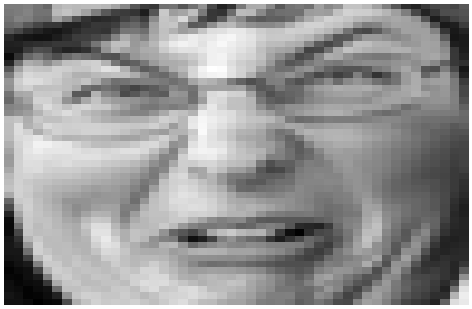
\includegraphics[width=0.15\linewidth]{images/sample_disgust.png}}
		\subfloat[Tristeza]{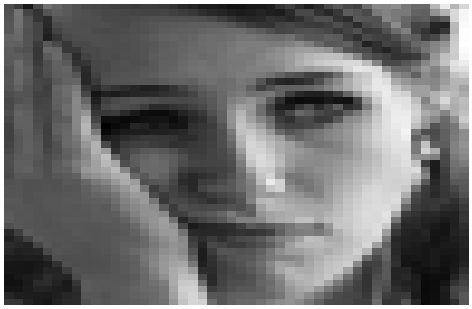
\includegraphics[width=0.15\linewidth]{images/sample_sad.png}}
	\end{tabular}

	\vspace{\floatsep}

  \begin{tabular}{@{}c@{}}
		\subfloat[Surpresa]{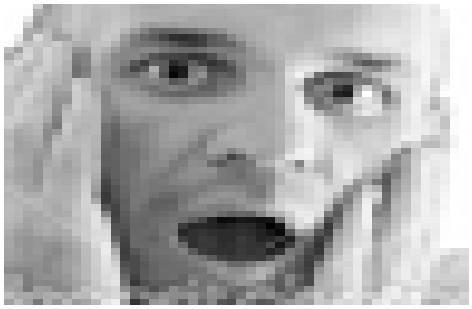
\includegraphics[width=0.15\linewidth]{images/sample_surprise.png}}
  	\subfloat[Medo]{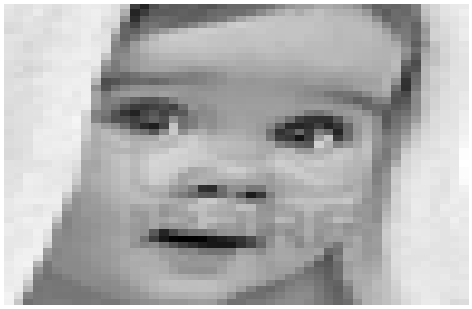
\includegraphics[width=0.15\linewidth]{images/sample_fear.png}}
  	\subfloat[Raiva]{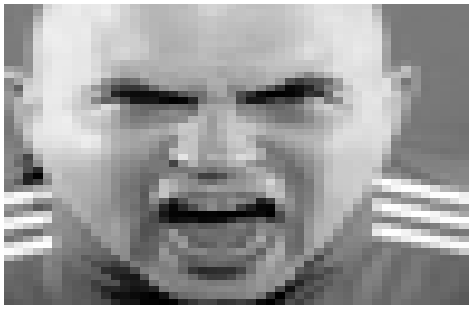
\includegraphics[width=0.15\linewidth]{images/sample_angry.png}}
    \subfloat[Neutro]{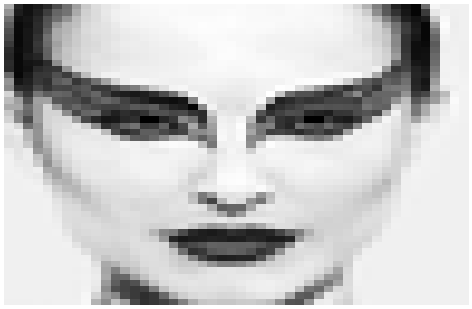
\includegraphics[width=0.15\linewidth]{images/sample_neutral.png}}
  \end{tabular}
\end{figure}

Conforme ilustra a Figura \ref{fig:samples}, é interessante notar algumas características particulares das imagens do FER2013 que ressaltam a relevância desta base de dados. Observa-se que, embora as faces estejam centralizadas nas imagens, elementos como cortes de cabelo, barba, óculos e até mesmo mãos encontram-se presentes, diminuindo a distância entre os exemplos contidos nesta base de dados e aqueles passíveis de ocorrência em um cenário realístico.

Os exemplos disponíveis na FER2013 se distribuem de maneira heterogênea perante as classes consideradas, conforme ilustra o gráfico da Figura \ref{fig:dataset}. O número de exemplos rotulado com a expressão ``nojo'', por exemplo, representam apenas $1.5\%$ do total de exemplos disponíveis. Estas características evidenciam o desbalanceamento do conjunto de dados considerado no tocante à quantidade de amostras por classe.

\begin{figure}[!htb]
    \centering
    \caption{Distribuição de imagens por tipo de expressão facial na base FER2013.}  \label{fig:dataset}
    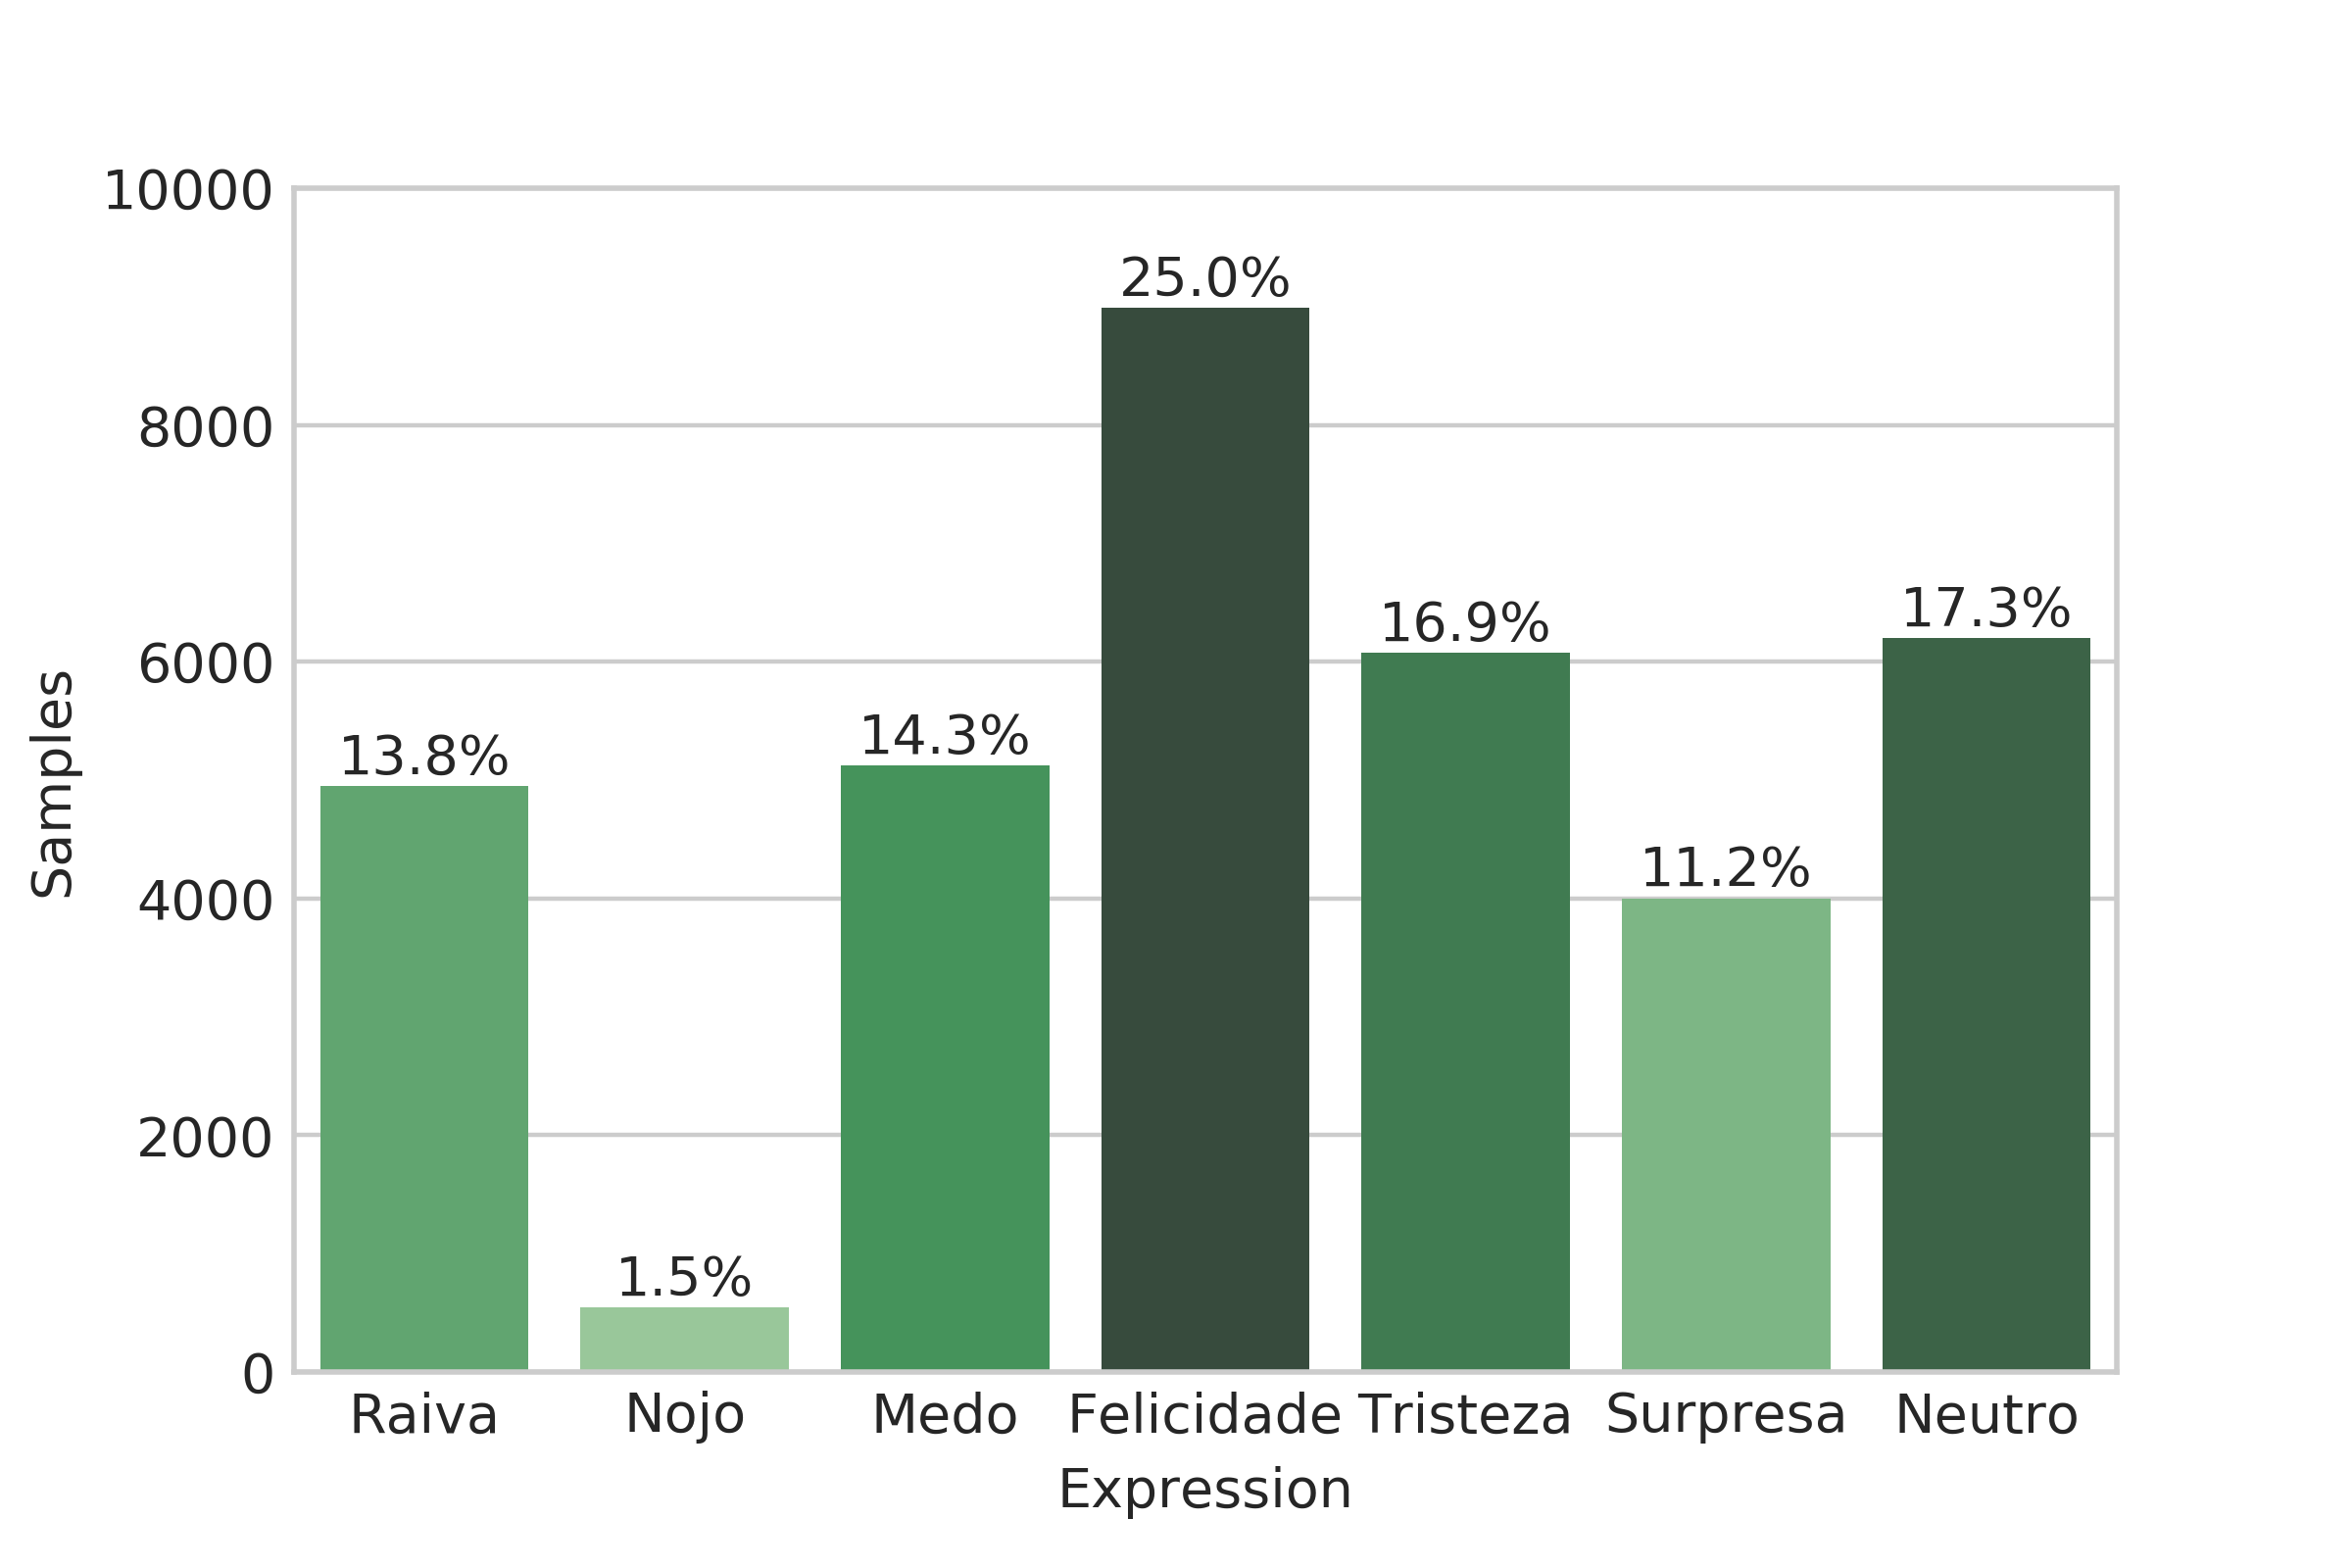
\includegraphics[width=10cm]{images/expression_distribution.png}
\end{figure}


\subsection{Descrição da Tarefa de Aprendizado de Máquina}
A base de dados em questão será usada para realização de tarefa de classificação multi-rótulo segundo o paradigma de aprendizado supervisionado. Nesta tarefa, exemplos de expressões faciais e seus respectivos rótulos serão fornecidos previamente aos modelos de Aprendizado de Máquina para escolha e ajuste de parâmetros e realização do treinamento. Posteriormente, expressões faciais ainda não vistas serão apresentadas e o objetivo será avaliar o desempenho do modelo na classificação destes exemplos, isto é, aferir a respectiva capacidade de generalização.

Obedecendo a uma partição do FER2013 previamente considerada em competições de Visão Computacional \cite{Kaggle:FER2013}, esta base de dados será dividida em $3$ partes, sendo: $80\%$ dos exemplos para treinamento,  $10\%$ dos exemplos para validação e $10\%$ dos exemplos remanescentes para testes, a serem utilizados seguindo uma abordagem de \emph{holdout} de validação cruzada  \cite{Brink:MachineLearningLivro}.  Apenas os exemplos da partição de testes serão utilizados para obtenção das métricas de desempenho e comparação dos modelos. Conforme ilustra a Figura \ref{fig:particoes}, as partições preservam a distribuição de amostras por classe na base de dados original.

\begin{figure}[h!]
	\centering
  	\caption{Distribuição das classes nas partições adotadas para o conjunto de dados.} \label{fig:particoes}
	\subfloat[Treinamento]{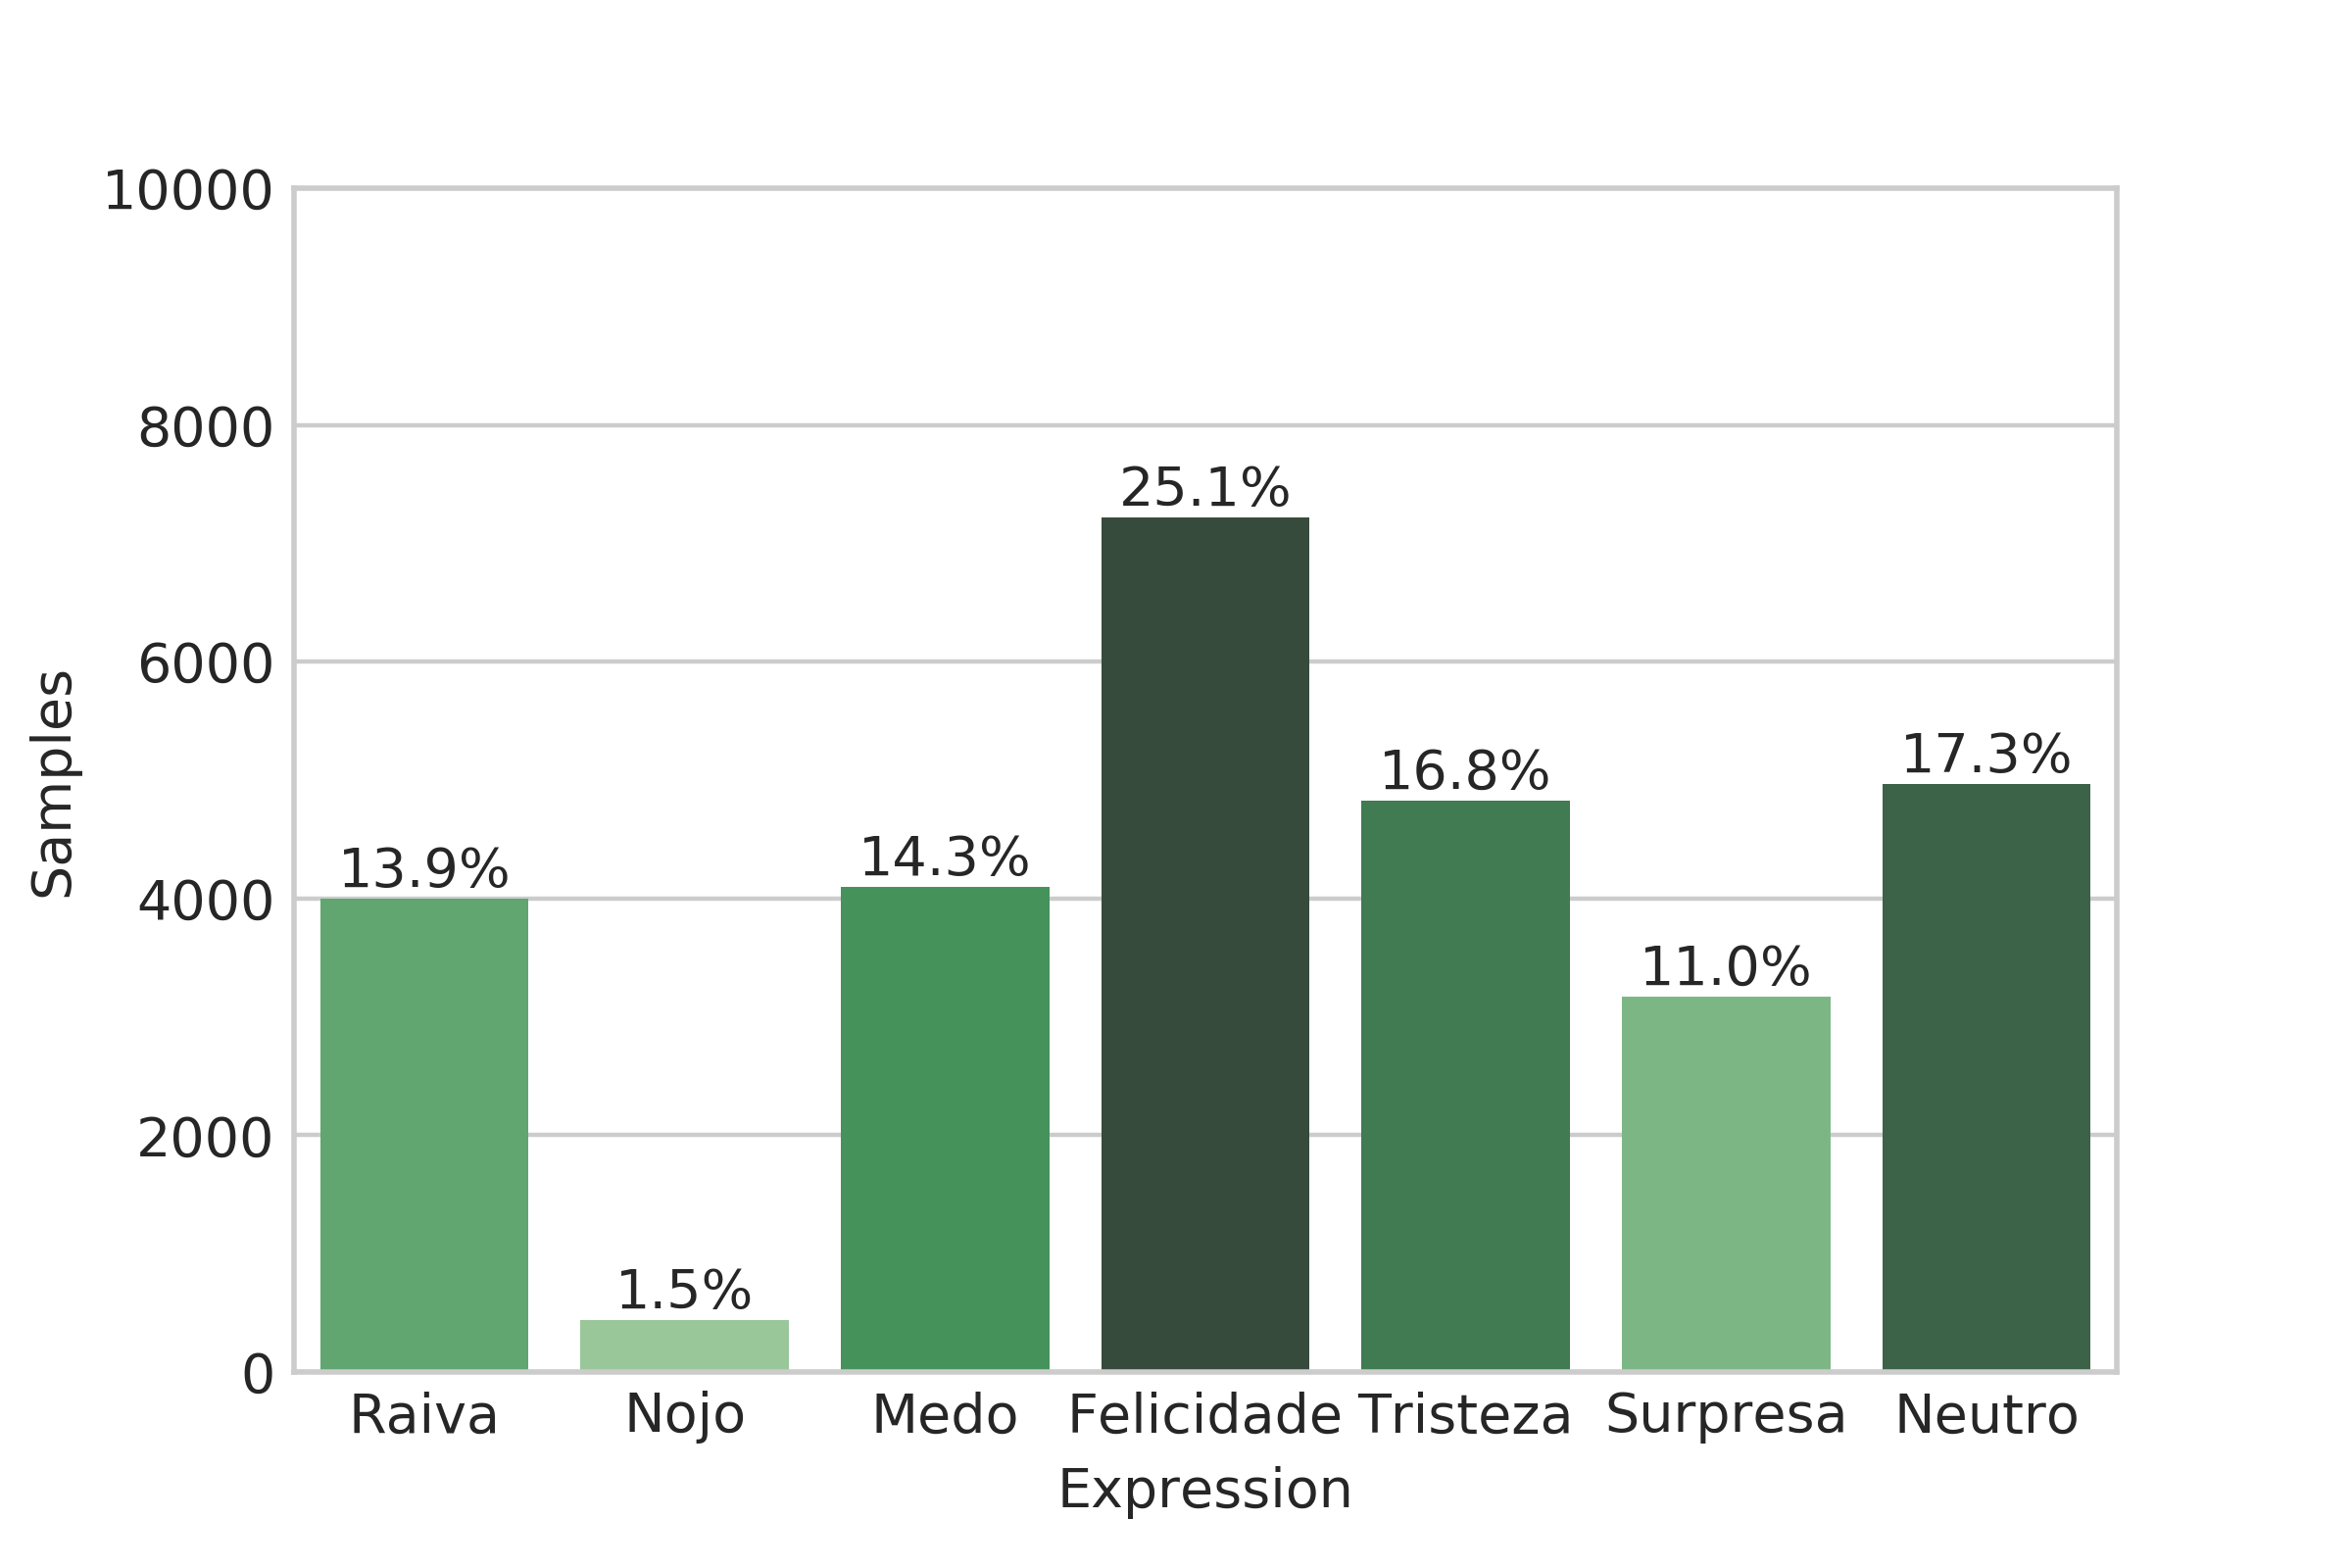
\includegraphics[width=0.33\linewidth]{images/expression_distribution_training.png}}
	\subfloat[Validação]{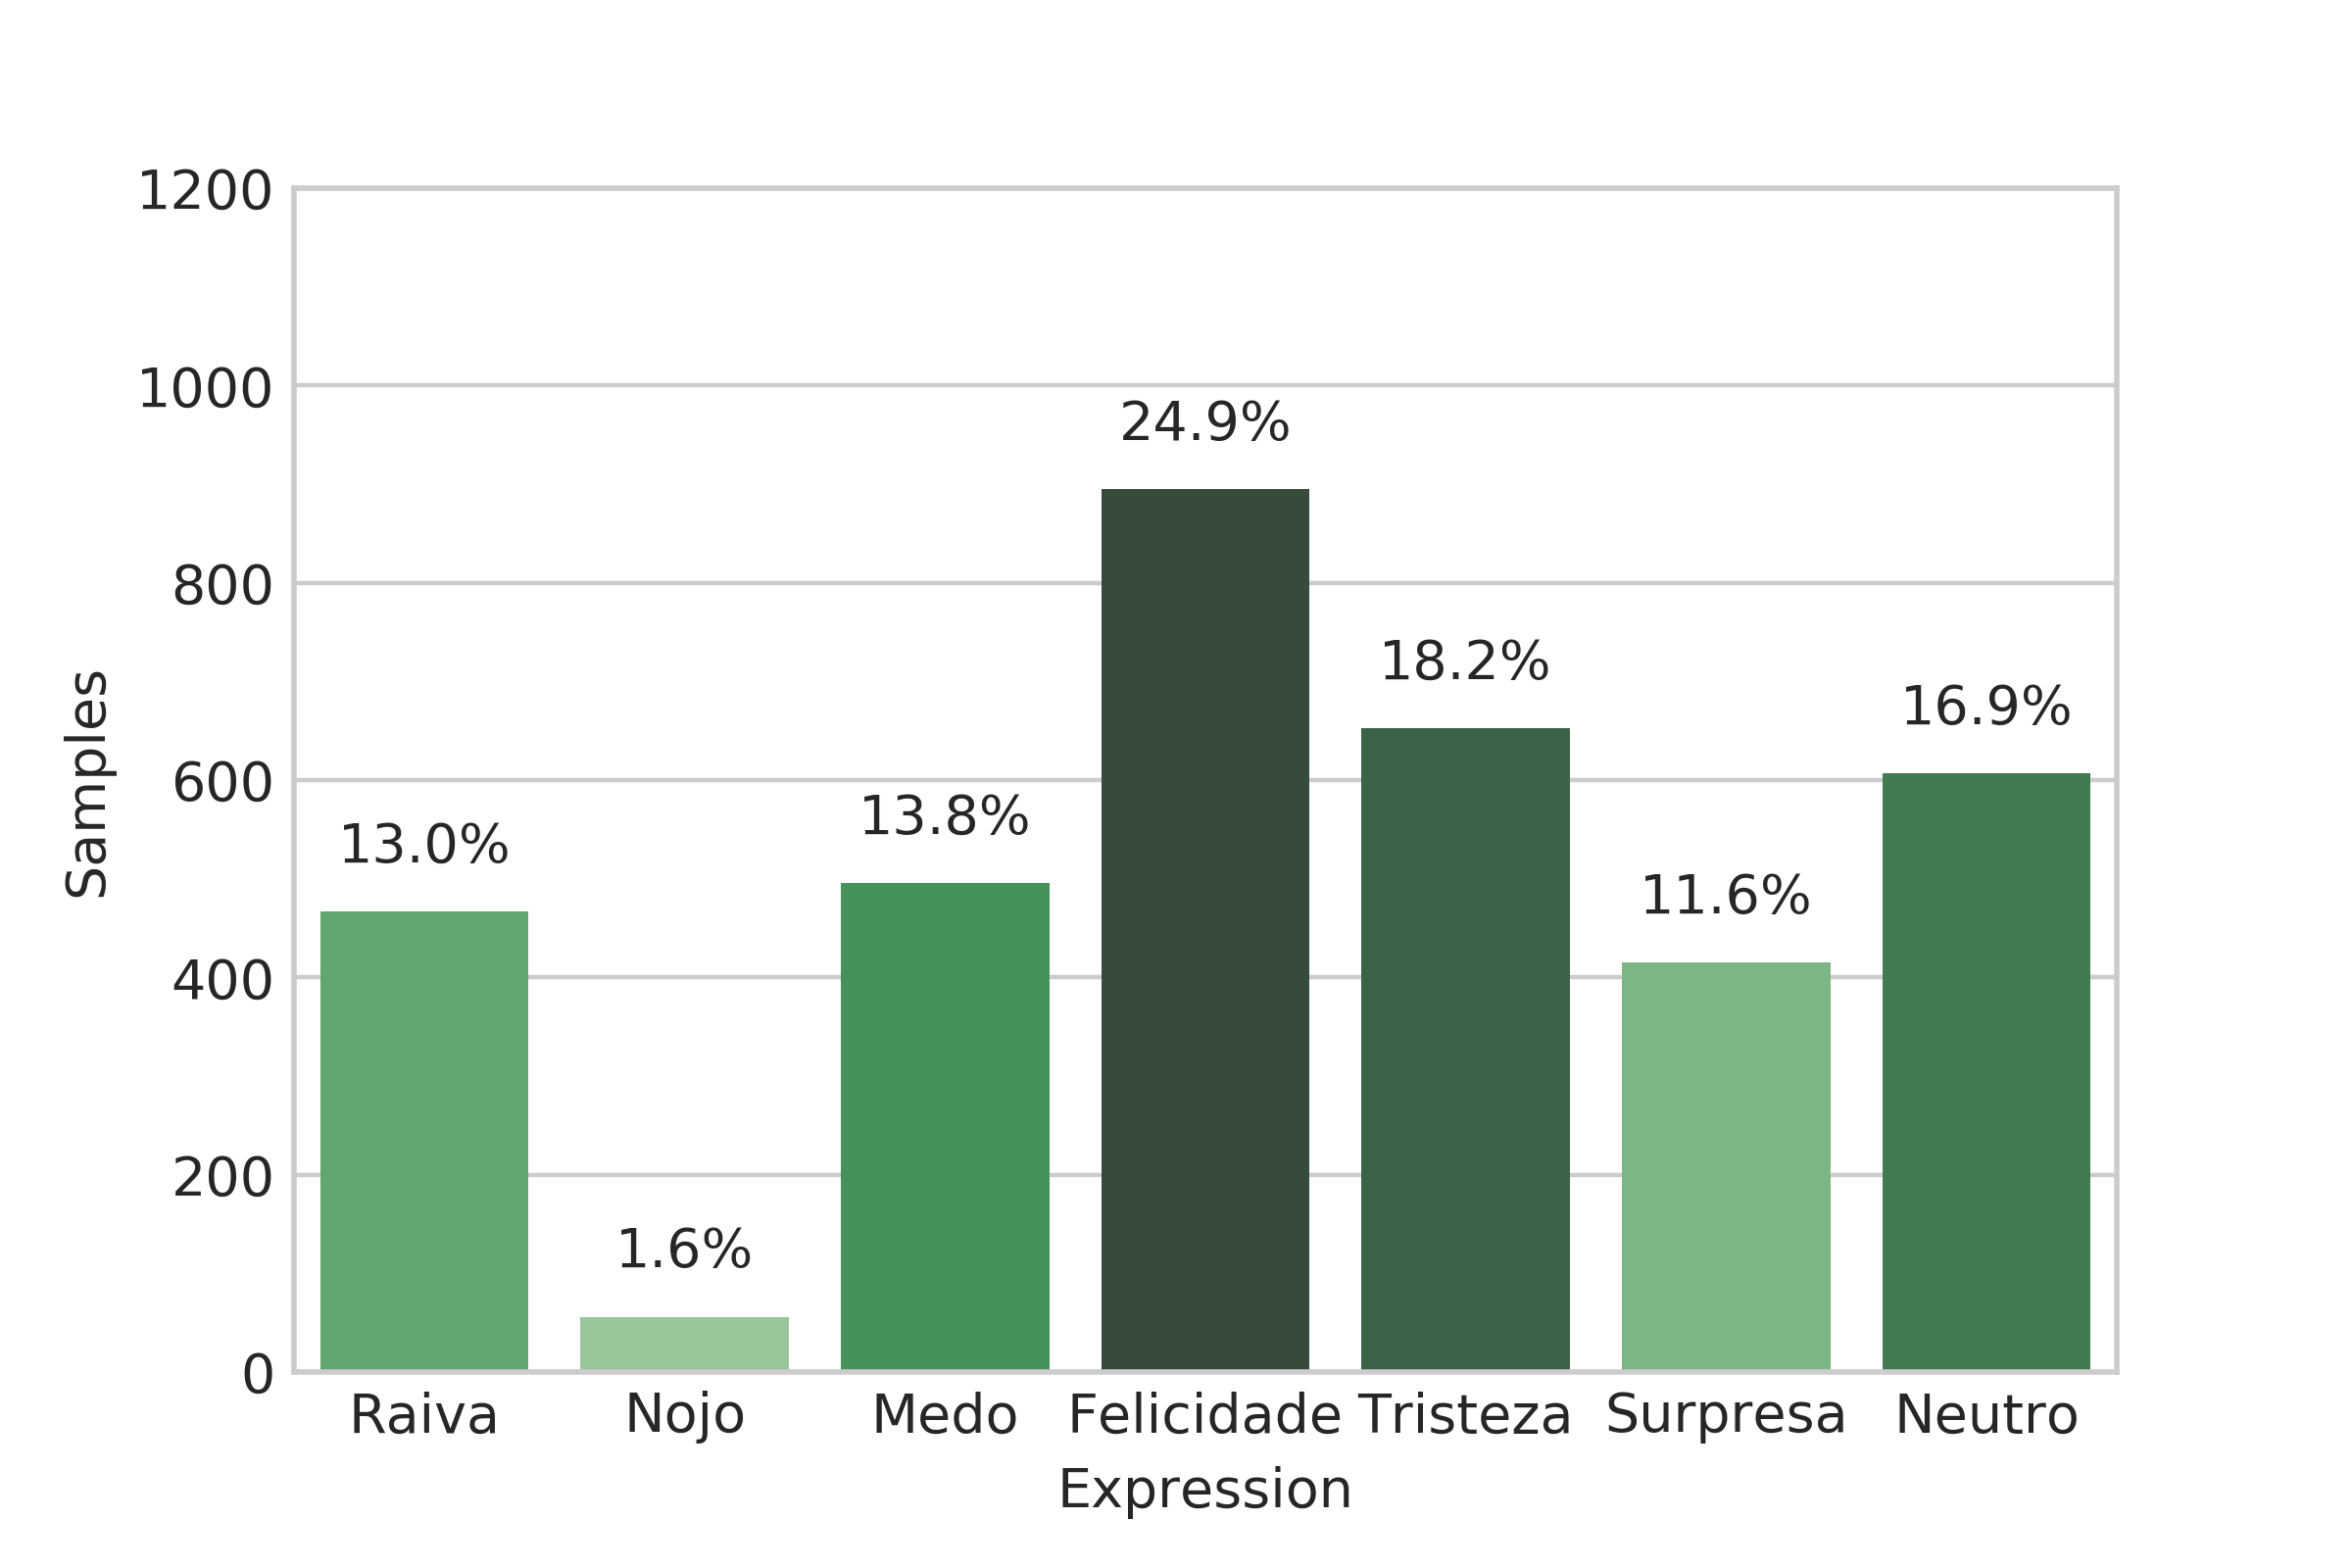
\includegraphics[width=0.33\linewidth]{images/expression_distribution_validation.png}}
	\subfloat[Teste]{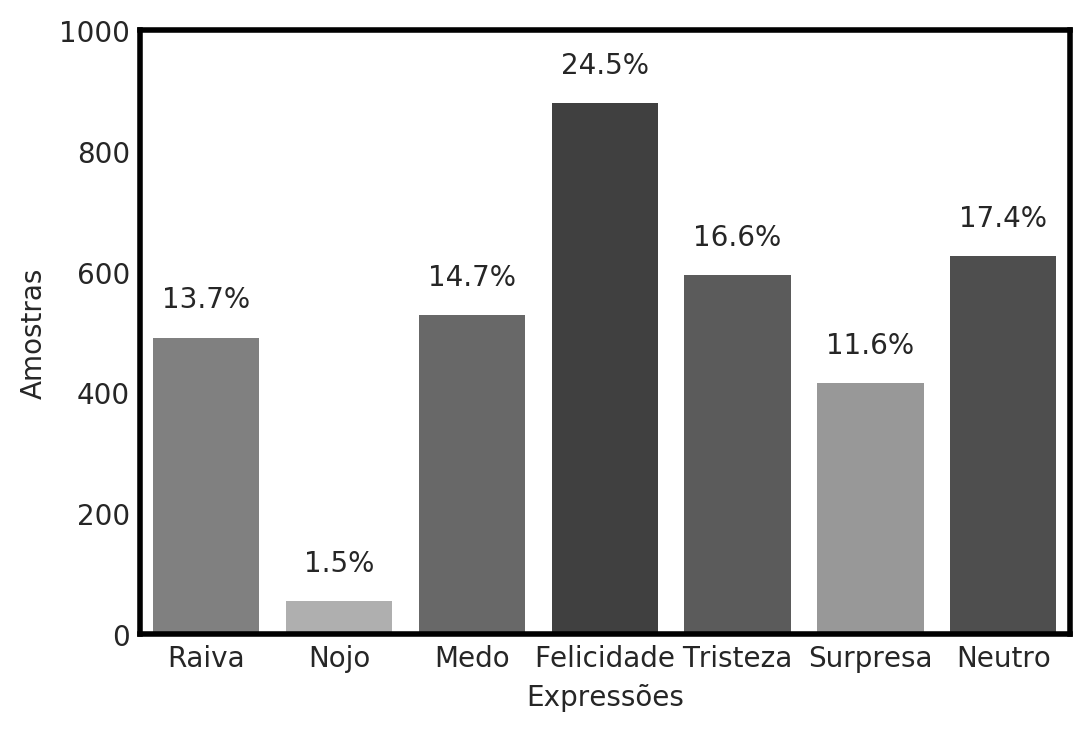
\includegraphics[width=0.33\linewidth]{images/expression_distribution_test.png}}
\end{figure}

Levando em conta os modelos de Aprendizagem de Máquina para a tarefa em questão, é essencial que um número razoável de exemplos esteja disponível para um ajuste apropriado dos parâmetros treináveis, pois com uma base de dados pequena estes ficam propensos a \textit{overfitting}, o que inibe a capacidade de generalização, em dados não vistos\cite{DBLP:journals/corr/abs-1708-06020}. Considerando esta necessidade prática, os exemplos da partição de treinamento passaram por um processo de pseudo-expansão do tipo \emph{data augmentation}, em que novas imagens foram geradas a partir das previamente existentes considerando transformações lineares de rotação, translação, escala e reflexão, colaborando para a posterior regularização dos modelos \cite{Chollet:Livro}, tornando-os invariantes aos tipos de operações realizadas\cite{DBLP:journals/corr/abs-1708-06020}. Que consistiram de rotação em módulo de até $10\textordmasculine$ no sentido horário e anti-horário, translações de até $10$ pixels nas direções ortogonais, fator de escala em módulo de $4$ e reflexão em relação ao eixo das ordenadas. Ao final desta etapa, o conjunto de treinamento passou a conter $1.33\times10^{15}$ exemplos, um aumento de $3.70\times10^{10}$ vezes em relação ao seu tamanho original, mas preservando a distribuição de exemplos nas classes.

A métrica de desempenho adotada para comparação dos modelos na realização desta tarefa foi o Micro $F$-\emph{Score}. Embora a acurácia seja uma métrica mais popular, que descreve o percentual de acertos do modelo em relação ao total de previsões efetuadas, não fornece detalhes acerca dos acertos por classe. Para contornar esta dificuldade, o Micro $F$-\emph{Score} foi preferido, pois contempla a média harmônica entre precisão e revocação por classe ao passo que considera as diferentes frequências nas classes do problema \cite{Kubat:Livro}. Esta métrica é especialmente utilizada em problemas de classificação com classes desbalanceadas, ou seja, em situações análogas ao cenário considerado no escopo deste trabalho.

Dentre os modelos a serem avaliados, serão elencados como mais aptos para a tarefa de classificação proposta aqueles que maximizarem a métrica de desempenho Micro $F$-\emph{Score}  para os exemplos pertencentes à partição de testes.


\subsection{Proposição de Modelos}
Os modelos propostos e seus respectivos parâmetros e hiperparâmetros para a tarefa de classificação de expressões faciais são descritos detalhadamente ao longo desta seção.

Seguindo a abordagem predominantemente adotada pelo estado da arte no tocante ao aprendizado de características em dados de alta dimensionalidade para tarefas de Visão Computacional \cite{Khan:Livro}, as redes neurais convolucionais foram o modelo de Aprendizado de Máquina adotado na tarefa elencada. Em particular, a arquitetura base foi a da rede neural convolucional canônica VGG-16 \cite{VGG}, mas com algumas adaptações. Esta arquietura originalmente proposta  destacou-se mediante a ideia de que uma rede neural precisa ter uma quantidade razoável  de camadas convolucionais profundas para uma representação hierárquica adequada das informações visuais.

As adaptações da VGG-16 levaram em conta diferentes quantidades de repetições de certas operações, apresentadas de acordo com a seguinte ideia geral:
\begin{equation}
\begin{split}
\textrm{Camada de Entrada} & \Rightarrow [ (\textrm{Convolução} \rightarrow \textrm{Batch Normalization})\cdot i\\
 &\quad \Rightarrow (\textrm{Pooling} \rightarrow \textrm{Dropout})\cdot j]\cdot k \\
 &\quad \Rightarrow [\textrm{Fully Connected} \rightarrow \textrm{ReLu}]\cdot \ell \\
 &\quad \Rightarrow \textrm{Flatten} \Rightarrow \textrm{Camada de Saída},
\end{split}
\end{equation} em que $i, j, k, \ell$ são números inteiros que denotam a quantidade de repetições da operação associada perante multiplicação. Os valores destes inteiros foram: $i = 2$, $j = \{1, \ldots, 5\}$, $k = \{2, 3, 4\}$ e $\ell = \{ 1,2,3 \}$.\ Considerando esta abordagem de adaptação, foram então propostas $9$ CNNs diferentes a serem treinadas e testadas, conforme a abordagem de validação cruzada previamente descrita.

% Complementar um pouco os parâmetros que você falou depois

Além da avaliação individual do desempenho das CNNs propostas, considerou-se também a posterior combinação destas redes em um \emph{ensemble}. Para valoração da classificação final, ao invés de considerar as abordagens típicas de votação unânime ou majoritária adotadas por \emph{ensembles}, utilizou-se um modelo baseado em \emph{Boosting}, o XGBoost \cite{Chen:Boosting}. Este modelo recebe as saídas de todas as redes individuais e, após ter sido treinado com os exemplos da base de dados, decide dentre as classificações individuais qual a classificação final mais apropriada. Observa-se aqui uma modificação não-trivial em \emph{ensembles}: a votação mediada por um modelo inteligente. A Figura X ilustra a ideia considerada.

\begin{figure}[!htb]
    \centering
    \caption{\emph{Ensemble} de CNNs com votação mediada por XGBoost.} \label{fig:ensemble}
    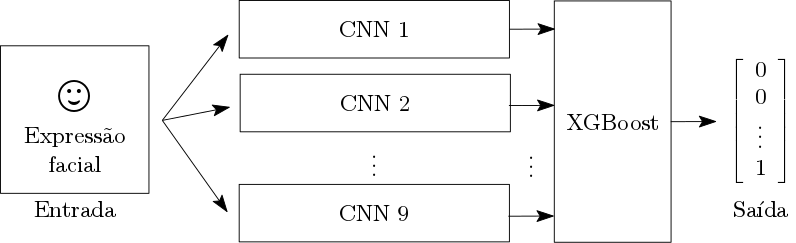
\includegraphics[width=0.9\textwidth]{images/ensemble-elloa.png}
\end{figure}



\iffalse
O modelo proposto consiste de um conjunto de \emph{Convolutional Neural Networks} (CNN), onde cada elemento é responsável pela classificação da imagem de entrada em uma das Sete Expressões Faciais Universais \cite{}, por meio da produção de vetor de probabilidades. Que consiste na possibilidade de cada uma das expressões universais estarem sendo expressas pela face, na imagem. A determinação da classificação final, não segue as abordagens típicas da literatura, via maioria ou consenso. Pois, estes vetores de probabilidades foram utilizados, de maneira supervisionada, para treinar um modelo do tipo \emph{XGBoost}, que finalmente atribui o rótulo mais adequado à entrada. Tem-se então um \emph{emsemble} de CNN com processo decisório de classificação realizado de maneira não trivial por um modelo de \emph{Machine Learning}.

O objetivo com a união de vários modelos de CNN foi obter classificadores bons de maneira geral em todas as expressões, contudo, estes deveriam se sobressair em determinadas expressões. Com isso, foram gerados sete modelos, um para cada expressão que deveriam ser classificadas, contudo, além dos sete classificadores bons individualmente na classificação de determinada expressão, adicionou-se dois outros, os quais obtiveram melhor desempenho considerando a classificação de todas as expressões, mas não obtiveram melhores resultados em determinada expressão em relação aos classificadores individuais.

Segundo \cite{}, o modelo \emph{XGBoost} é um bom modelo para se utilizar na técnica \emph{Boost}, que tem como objetivo obter um modelo \emph{Stronger} baseado nas combinações das respostas de \emph{Weak Learners}. Visto isso, foi considerado cada modelo de CNN, como um \emph{Weak Learner}, apesar de eles não serem fracos, dada a complexidade da tarefa e seus resultado, Tabela \ref{tbl:fscore}. E como saída estes forneciam seus resultados, vetores de probabilidade, para o modelo \emph{XGBoost} que tratava de melhor combinar os resultados individuais para se obter um melhor resultado de predição.

As arquiteturas CNN utilizadas na construção do modelo, foram baseadas na arquitetura \emph{VGG-16} \cite{}, que consiste de camadas duplas ou triplas de convolução 2D, com \emph{kernel} de 3x3, seguidas de \emph{pooling}, utilizando \emph{MaxPooling}. E como saída tem camadas densas, também chamadas de \emph{Fully Connected} (FC), onde a última utiliza a função de ativação \emph{SoftMax}.

Como função de ativação para as camadas convolucionais e densas, foi utilizada a função \emph{ReLU}, devido ao seu baixo custo computacional, e também possuir derivada constante, o que contribui para o desempenho da função de otimização \emph{adam} \cite{}. Segundo \cite{}, e análise experimental, a inicialização dos pesos iniciais das camadas convolucionais que utilizam a função de ativação \emph{ReLu}, com o inicializador de He et al \cite{}, possibilita aumento no desempenho, convergência, durante o treinamento dos modelos CNN.

Após a saída de cada camadas convolucionais, foi utilizada normalização em lotes, \emph{Batch Normalization}, pois, segundo \cite{} e análise experimental, os modelos modelos de CNN possuem melhores resultados nas predições, tanto na etapa de treinamento quanto na etapa de generalização.

Algumas das "regras de ouro" \cite{} para construção de modelos baseados em \emph{Artificial Neural Networks} (ANN) foram utilizadas nas camadas densas, visto que estas são equivalentes. Foram elas: A quantidade de neurônios das cadas ocultas não deve ultrapassar o dobro da quantidade dados da entrada, e a quantidade de neurônios da camada de entrada deve ser a mesma da quantidade de dados da entrada. Vale ressaltar, que as camadas de \emph{FC} em sua maioria não possuem mais do que duas camadas ocultas, devido ao Teorema de aproximação universal \cite{}.

Para regularização dos modelos de CNN foi utilizado somente \emph{Dropout}, visto que os regularizadores $l1$ e $l2$, não apresentaram bons resultados durante o período de treinamento, o que tornavam o modelo instável ou com tendências a \emph{underfitting}. Essa tendência foi evidenciada pelo desempenho constante do modelo por algumas dezenas de épocas de treinamento, e ao ser percebido esse comportamento o treinamento foi interrompido.

A arquitetura final dos modelos de CNN podem ser visualizados na Tabela \ref{tbl:arch}. Já a arquitetura utilizada pelo \emph{XGBoost} não pode ser mostrada, devido a esta ter mil árvores classificadoras, o que torna inviável a apresentação desta neste artigo.

\begin{table}
\centering
\caption{Arquiteturas utilizadas}
\label{tbl-arch}
\resizebox{\textwidth}{!}{%
\begin{tabular}{@{}lllllllll@{}}
\toprule
\multicolumn{1}{c}{1} & \multicolumn{1}{c}{2} & \multicolumn{1}{c}{3} & \multicolumn{1}{c}{4} & \multicolumn{1}{c}{5} & \multicolumn{1}{c}{6} & \multicolumn{1}{c}{7} & \multicolumn{1}{c}{8} & \multicolumn{1}{c}{9} \\ \midrule
Conv2D\_(64, 3, 3)    & Conv2D\_(64, 3, 3)    & Conv2D\_(64, 3, 3)    & Conv2D\_(64, 3, 3)    & Conv2D\_(64, 3, 3)    & Conv2D\_(64, 3, 3)    & Conv2D\_(128, 7, 7)   & Conv2D\_(16, 7, 7)    & Conv2D\_(16, 7, 7)    \\
BatchNorm             & BatchNorm             & BatchNorm             & BatchNorm             & BatchNorm             & BatchNorm             & BatchNorm             & BatchNorm             & BatchNorm             \\
Conv2D\_(64, 3, 3)    & Conv2D\_(64, 3, 3)    & Conv2D\_(64, 3, 3)    & Conv2D\_(64, 3, 3)    & Conv2D\_(64, 3, 3)    & Conv2D\_(64, 3, 3)    & Conv2D\_(128, 7, 7)   & Conv2D\_(16, 7, 7)    & Conv2D\_(16, 7, 7)    \\
BatchNorm             & BatchNorm             & BatchNorm             & BatchNorm             & BatchNorm             & BatchNorm             & BatchNorm             & BatchNorm             & BatchNorm             \\
MaxPool\_(3, 3)       & MaxPool\_(3, 3)       & MaxPool\_(3, 3)       & MaxPool\_(3, 3)       & MaxPool\_(3, 3)       & MaxPool\_(3, 3)       & AvgPool\_(3, 3)       & AvgPool\_(3, 3)       & AvgPool\_(3, 3)       \\
Dropout\_50           & Dropout\_50           & Dropout\_50           & Dropout\_50           & Dropout\_50           & Dropout\_50           & Dropout\_50           & Dropout\_50           & Dropout\_50           \\
Conv2D\_(128, 3, 3)   & Conv2D\_(128, 3, 3)   & Conv2D\_(128, 3, 3)   & Conv2D\_(128, 3, 3)   & Conv2D\_(128, 3, 3)   & Conv2D\_(128, 3, 3)   & Conv2D\_(128, 5, 5)   & Conv2D\_(32, 3, 3)    & Conv2D\_(32, 3, 3)    \\
BatchNorm             & BatchNorm             & BatchNorm             & BatchNorm             & BatchNorm             & BatchNorm             & BatchNorm             & BatchNorm             & BatchNorm             \\
Conv2D\_(128, 3, 3)   & Conv2D\_(128, 3, 3)   & Conv2D\_(128, 3, 3)   & Conv2D\_(128, 3, 3)   & Conv2D\_(128, 3, 3)   & Conv2D\_(128, 3, 3)   & Conv2D\_(128, 5, 5)   & Conv2D\_(32, 3, 3)    & Conv2D\_(32, 3, 3)    \\
BatchNorm             & BatchNorm             & BatchNorm             & BatchNorm             & BatchNorm             & BatchNorm             & BatchNorm             & BatchNorm             & BatchNorm             \\
MaxPool\_(3, 3)       & MaxPool\_(3, 3)       & MaxPool\_(3, 3)       & MaxPool\_(3, 3)       & MaxPool\_(3, 3)       & MaxPool\_(3, 3)       & AvgPool\_(3, 3)       & AvgPool\_(3, 3)       & AvgPool\_(3, 3)       \\
Dropout\_50           & Dropout\_50           & Dropout\_50           & Dropout\_50           & Dropout\_50           & Dropout\_50           & Dropout\_50           & Dropout\_50           & Dropout\_50           \\
Conv2D\_(256, 3, 3)   & Conv2D\_(256, 3, 3)   & Conv2D\_(256, 3, 3)   & Conv2D\_(256, 3, 3)   & Conv2D\_(256, 3, 3)   & Conv2D\_(256, 3, 3)   & Conv2D\_(256, 3, 3)   & Conv2D\_(64, 3, 3)    & Conv2D\_(64, 3, 3)    \\
BatchNorm             & BatchNorm             & BatchNorm             & BatchNorm             & BatchNorm             & BatchNorm             & BatchNorm             & BatchNorm             & BatchNorm             \\
Conv2D\_(256, 3, 3)   & Conv2D\_(256, 3, 3)   & Conv2D\_(256, 3, 3)   & Conv2D\_(256, 3, 3)   & Conv2D\_(256, 3, 3)   & Conv2D\_(256, 3, 3)   & Conv2D\_(256, 3, 3)   & Conv2D\_(64, 3, 3)    & Conv2D\_(64, 3, 3)    \\
BatchNorm             & BatchNorm             & BatchNorm             & BatchNorm             & BatchNorm             & BatchNorm             & BatchNorm             & BatchNorm             & BatchNorm             \\
Conv2D\_(256, 3, 3)   & Conv2D\_(256, 3, 3)   & Conv2D\_(256, 3, 3)   & Conv2D\_(256, 3, 3)   & MaxPool\_(3, 3)       & Conv2D\_(256, 3, 3)   & AvgPool\_(3, 3)       & AvgPool\_(3, 3)       & AvgPool\_(3, 3)       \\
BatchNorm             & BatchNorm             & BatchNorm             & BatchNorm             & Dropout\_50           & BatchNorm             & Dropout\_50           & Dropout\_50           & Dropout\_50           \\
MaxPool\_(3, 3)       & MaxPool\_(3, 3)       & MaxPool\_(3, 3)       & MaxPool\_(3, 3)       & Flatten               & MaxPool\_(3, 3)       & Conv2D\_(256, 3, 3)   & Conv2D\_(128, 3, 3)   & Conv2D\_(128, 3, 3)   \\
Dropout\_50           & Dropout\_50           & Dropout\_50           & Dropout\_50           & FC\_(128)             & Dropout\_50           & BatchNorm             & BatchNorm             & BatchNorm             \\
Conv2D\_(512, 3, 3)   & Flatten               & Flatten               & Flatten               & Dropout\_20           & Flatten               & Conv2D\_(256, 3, 3)   & Conv2D\_(128, 3, 3)   & Conv2D\_(128, 3, 3)   \\
BatchNorm             & FC\_(128)             & FC\_(512)             & FC\_(128)             & FC\_(64)              & FC\_(128)             & BatchNorm             & BatchNorm             & BatchNorm             \\
Conv2D\_(512, 3, 3)   & Dropout\_20           & Dropout\_50           & Dropout\_20           & Dropout\_20           & Dropout\_20           & AvgPool\_(3, 3)       & AvgPool\_(3, 3)       & AvgPool\_(3, 3)       \\
BatchNorm             & FC\_(64)              & FC\_(512)             & FC\_(64)              & FC\_(32)              & FC\_(64)              & Dropout\_50           & Dropout\_50           & Dropout\_50           \\
Conv2D\_(512, 3, 3)   & Dropout\_20           & Dropout\_50           & Dropout\_20           & Dropout\_20           & Dropout\_20           & Flatten               & Flatten               & Flatten               \\
BatchNorm             & FC\_(7)               & FC\_(7)               & FC\_(7)               & FC\_(7)               & FC\_(32)              & FC\_(1048)            & FC\_(512)             & FC\_(512)             \\
MaxPool\_(3, 3)       &                       &                       &                       &                       & Dropout\_20           & Dropout\_20           & Dropout\_20           & Dropout\_50           \\
Dropout\_50           &                       &                       &                       &                       & FC\_(7)               & FC\_(512)             & FC\_(512)             & FC\_(512)             \\
Conv2D\_(512, 3, 3)   &                       &                       &                       &                       &                       & Dropout\_20           & Dropout\_20           & Dropout\_20           \\
BatchNorm             &                       &                       &                       &                       &                       & FC\_(7)               & FC\_(7)               & FC\_(7)               \\
Conv2D\_(512, 3, 3)   &                       &                       &                       &                       &                       &                       &                       &                       \\
BatchNorm             &                       &                       &                       &                       &                       &                       &                       &                       \\
Conv2D\_(512, 3, 3)   &                       &                       &                       &                       &                       &                       &                       &                       \\
BatchNorm             &                       &                       &                       &                       &                       &                       &                       &                       \\
MaxPool\_(3, 3)       &                       &                       &                       &                       &                       &                       &                       &                       \\
Dropout\_50           &                       &                       &                       &                       &                       &                       &                       &                       \\
Flatten               &                       &                       &                       &                       &                       &                       &                       &                       \\
FC\_(512)             &                       &                       &                       &                       &                       &                       &                       &                       \\
Dropout\_20           &                       &                       &                       &                       &                       &                       &                       &                       \\
FC\_(512)             &                       &                       &                       &                       &                       &                       &                       &                       \\
Dropout\_20           &                       &                       &                       &                       &                       &                       &                       &                       \\
FC\_(7)               &                       &                       &                       &                       &                       &                       &                       &                       \\ \bottomrule
\end{tabular}%
}
\end{table}

% TODO: Lembrar de falar da infra-estrutura para execução.
\fi



\section{Resultados e Discussões}
Nesta seção são apresentados os resultados obtidos na metodologia proposta em classificar automaticamente expressões faciais, com base na partição de teste. Em seguida, é analisado o desempenho dos componentes do \textit{Ensemble} na medida Micro \textit{F1 Score}, para cada expressão e por fim  é feita um comparativo com os resultados de trabalhos relacionados. \todo{Citar resultados de trabalhos relacionados}

\subsection{4.1 Classificação das Expressões Faciais}
Para executar a avaliação do modelo proposto na tarefa de classificação, aplicou-se os exemplos contidos na partição de teste, de forma sequencial e supervisionada. Onde o rótulo fornecido pelo modelo para cada exemplo foi armazendo como resultado predito, para futura comparação com o rótulo verdadeiro, que é o contido na base dados.

Após o processo de rotulação das amostras de teste pelo modelo, foram fornecidas as informações de dados rotulados, juntamente dos rótulos verdadeiros, a medida Micro \textit{F1 Score}, onde obteve-se como resultado o valor de $71.74$\%. Contudo, os trabalhos relacionados aqui apresentados fazem uso da medida de acurácia como resultados de desempenho, a qual foi obtida pelo mesmo método da medida Micro \textit{F1 Score}, e resultou em $71.74$\%.


\subsection{4.2 Desempenho dos componentes do \textit{Ensemble}}
O método utilizado para obtenção dos valores de Micro \textit{F1 Score} e acurácia para o \textit{Ensemble} foi o mesmo utilizado para os modelos de Rede Convolucional e \textit{Xtreme Gradient Boosting}. Ressaltando que os resultados das medidas de desempenho obtiveram os mesmos valores, sendo este o motivo de serem apresentados somente o valor da medida Micro \textit{F1 Score}. Na Tabela \ref{tbl:fscore} observa-se os resultados para cada modelo de Rede Convolucional, juntamente do resultado do \textit{Ensemble}.

\begin{table}[!htb]
\centering
\caption{F1 Micro das Arquiteturas utilizadas}
\label{tbl:fscore}
\begin{tabular}{@{}cc@{}}
\toprule
Modelo & F1 Micro           \\ \midrule
1      & 0.6898857620507105 \\
2      & 0.6767901922541097 \\
3      & 0.6606297018668152 \\
4      & 0.6798551128448036 \\
5      & 0.6667595430482028 \\
6      & 0.6781833379771524 \\
7      & 0.694901086653664  \\
8      & 0.6285873502368348 \\
9      & 0.6244079130677069 \\ 
ensemble & 0.7174700473669546 \\ \bottomrule
\end{tabular}
\end{table}

É observado que o melhor classificador, modelo 7, individual de CNN, obteve 69.49\% enquanto que o pior, modelo 9, obteve 62.44\%. Ressaltando que cada classificador de CNN usado no \emph{Ensemble} obteve resultados melhores do que os outros, em determinada expressão ou bons resultados em todas as expressões, mas não se sobressaiu em nenhuma expressão específica. No caso do modelo 9, obteve-se bons resultados em quase todas as expressões, mas nenhum resultado melhor na classificação de determinada expressão em relação aos outros modelos. Já no caso do modelo 7, obteve-se o melhor resultado de classificação para expressão de surpresa.

No modelo \textit{Ensemble} teve-se um total de 32.738.871 parâmetros treináveis, que é resultado da soma dos parâmetros treináveis dos modelos CNN, bem como do XGBoost. Onde o modelo de XGBoost possui uma quantidade pequena de parâmetros treináveis, em comparação com os modelos de CNN, pois, enquanto a quantidade deste está na ordem de milhares, os outros estão na ordem de milhões. Este comportamento se mostra coerente, se for levado em consideração as tarefas de cada modelo, que possuem complexidades bastante distintas.

Os modelos de CNN mais profundos, consequentemente com maior número de parâmetros treináveis, foram os que obtiveram melhores desempenho individuais.   Já os modelos mais rasos, apesar de obterem desempenho abaixo dos profundos, obtiveram os melhores resultados em classificar expressões específicas. Quantidade de parâmetros treináveis do \textit{Ensemble} podem ser visualizados na Tabela \ref{tbl:fscore}.

Na Figura \ref{fig:emsemble} é apresentado o resultado do modelo utilizando \emph{Ensemble}. Onde o resultado final de desempenho foi de 71.74\% de acordo com a métrica \emph{F1 Micro}, ressaltando que seu valor de Acurácia possui o mesmo valor. E com este resultado o \emph{Ensemble} supera, por pouco, o modelo campeão da competição.

\begin{figure}[!htb]
    \centering
    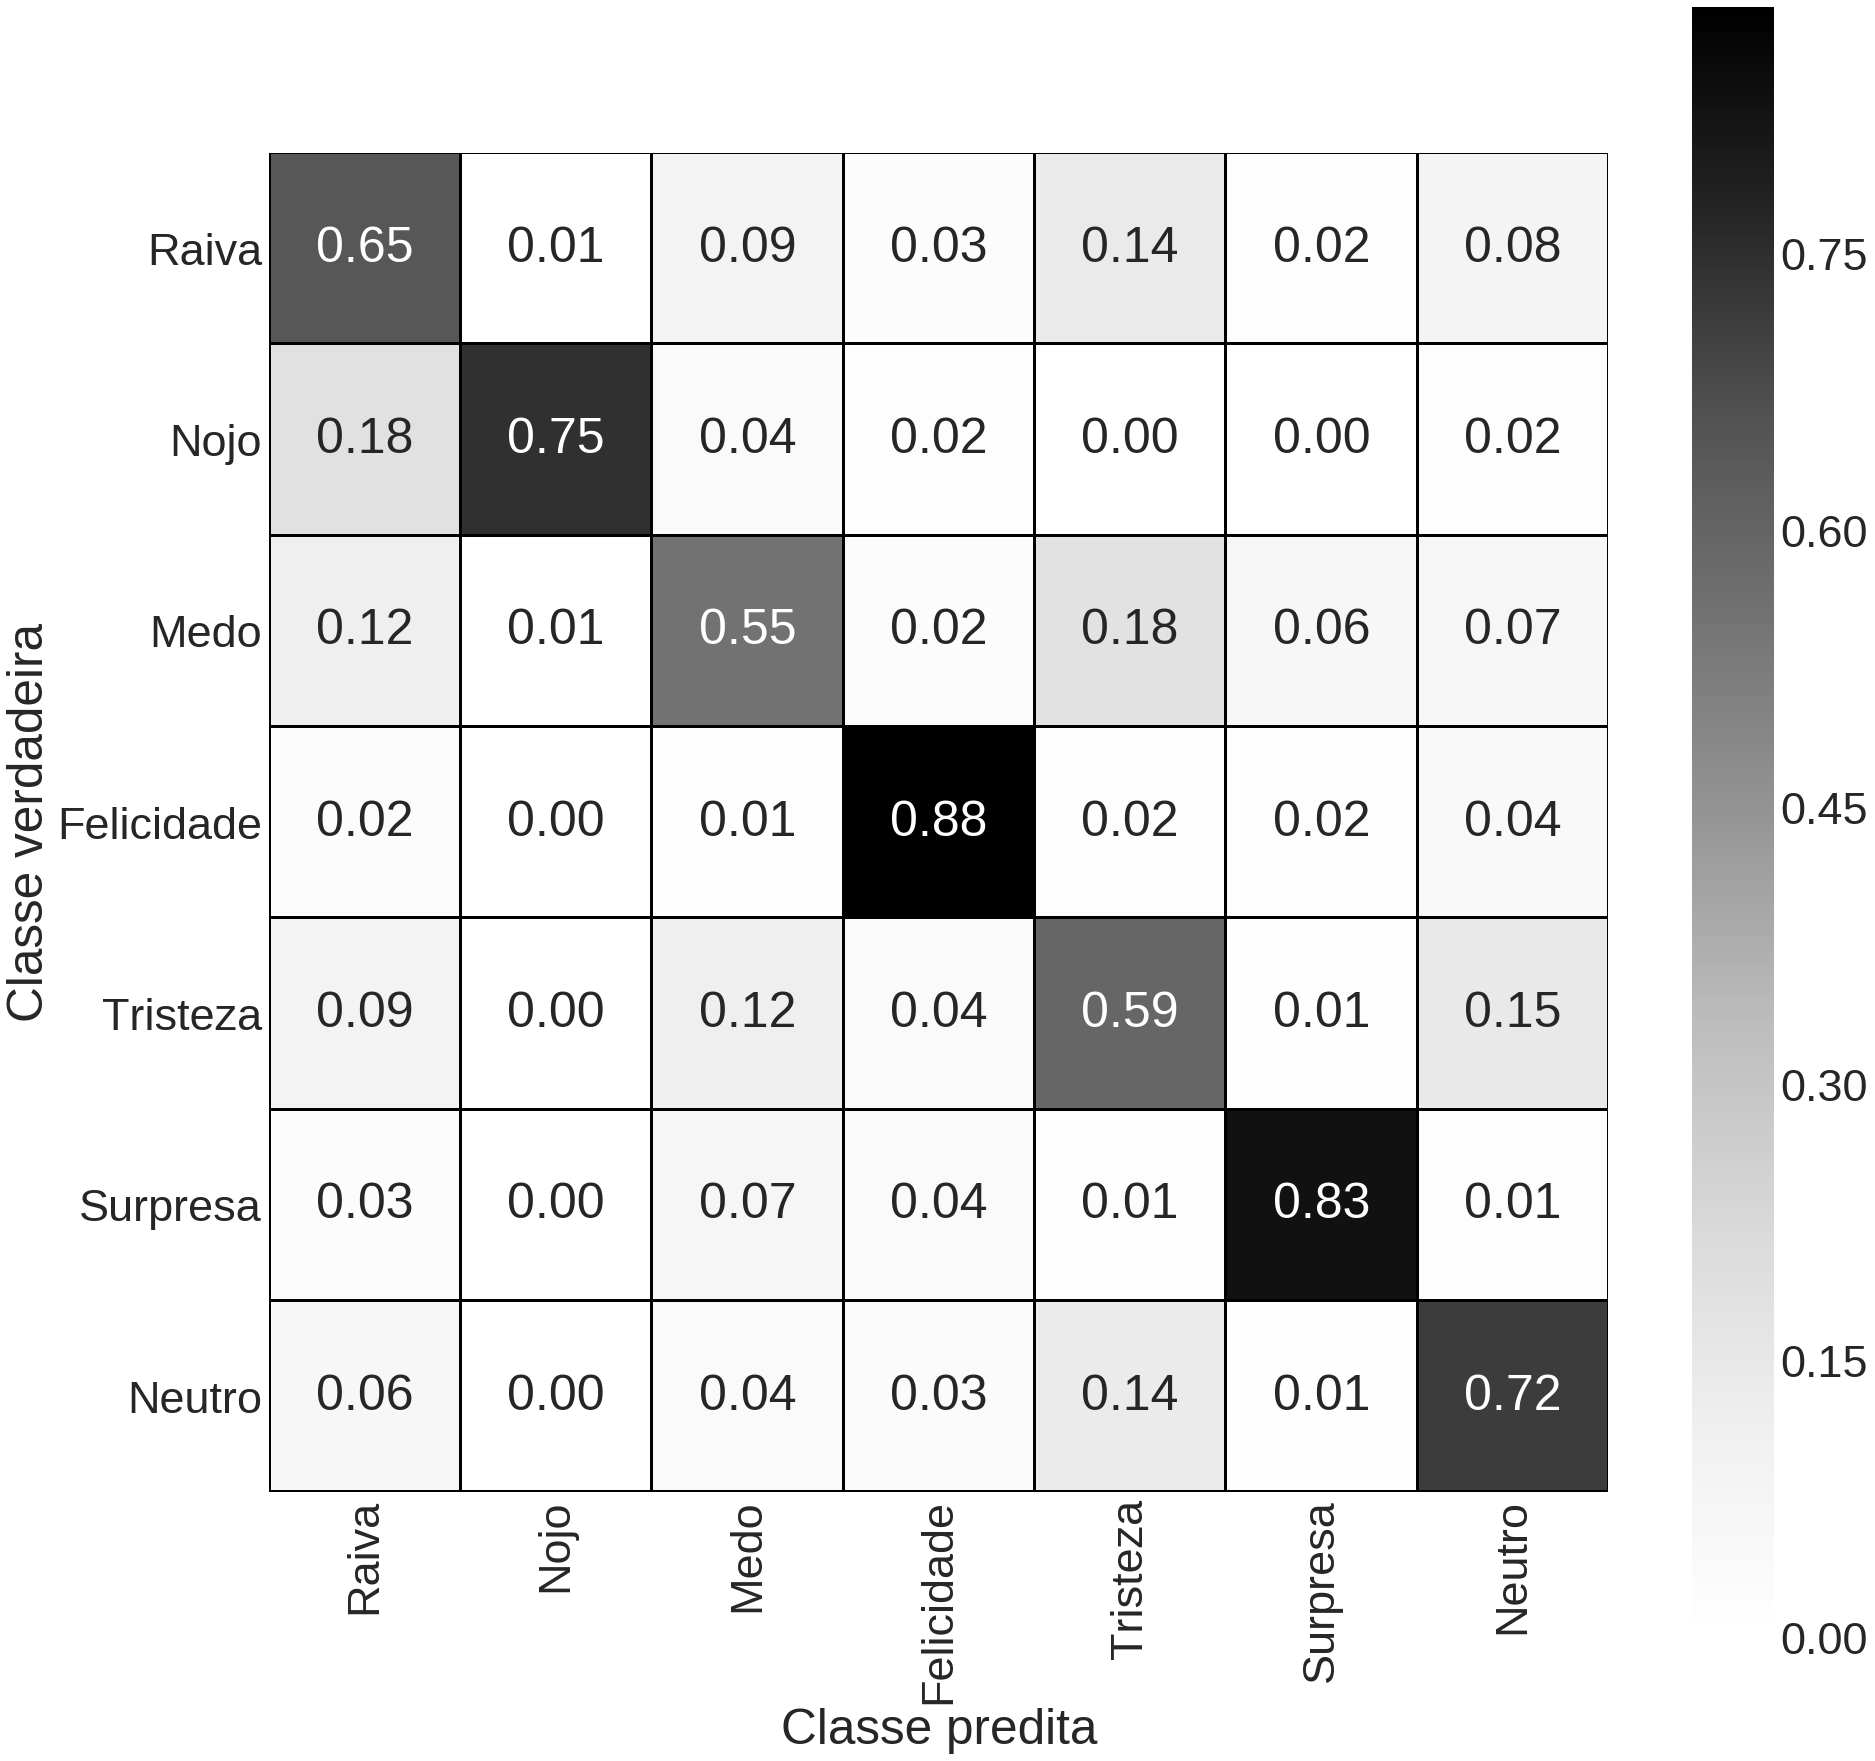
\includegraphics[width=9cm]{images/cm_emsemble.png}
    \caption{Matriz de Confusão do \emph{Ensemble} (CNN + \emph{XGBoost})}
    \label{fig:emsemble}
\end{figure}

Apesar do desbalanceamento da base de dados, a classificação da expressão de nojo obteve-se um dos melhores resultados \ref{fig:samples}, acompanhadas de surpresa e felicidade, com \textit{F1 Score} de
78\%, 83\%, e 89\% respectivamente. As classificações das outras expressões também apresentaram bons resultados, todas com \textit{F1 Score} maior ou igual a 58\%.

\begin{figure}[!htb]
    \centering
    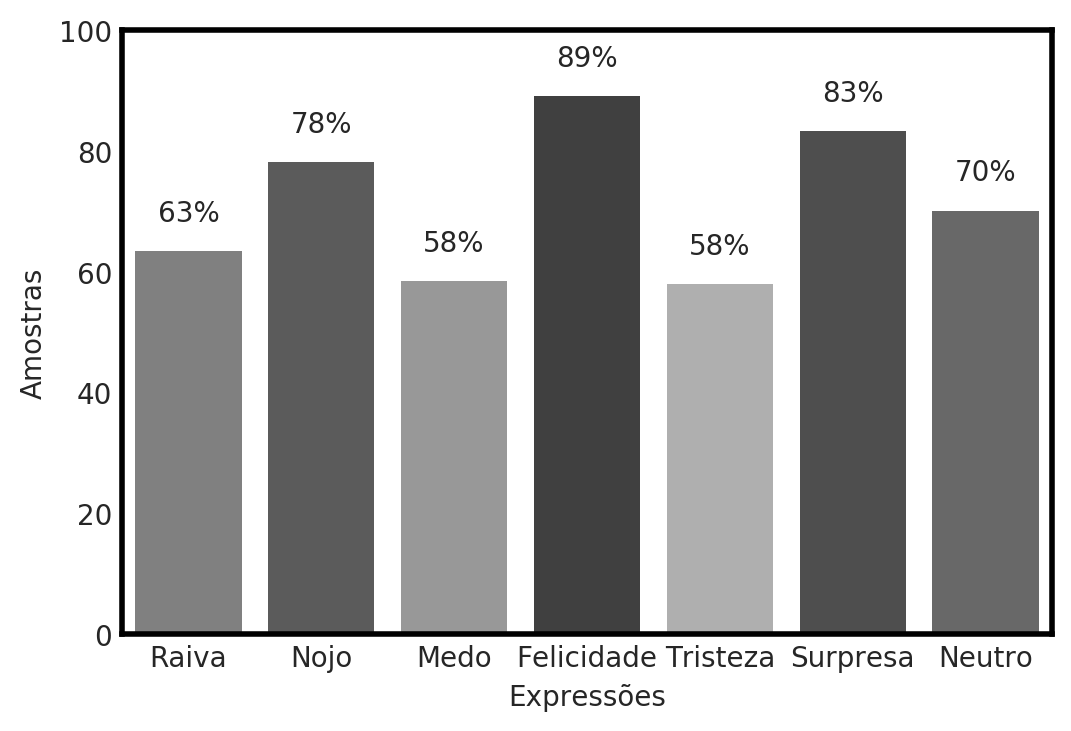
\includegraphics[width=8cm]{images/f1_bar.png}
    \caption{F1 Score por Expressão}
    \label{fig:f1_bar}
\end{figure}


\subsection{4.3 Comparativo de resultados com a literatura}



O modelo proposto conseguiu superar os seres humanos nesta base de dados, na tarefa de classificar as expressões faciais, visto que sua acurácia foi de $71.74$\%, enquanto a dos seres humanos é de $65\pm5$\% \cite{goodfellow2013challenges}.


\section{Considerações Finais}
\section{Conclusão}
Texto

% TODO - Alterar título das referências de References para Referências
% TODO - Alterar título das Figuras de Figure para Figuras
% TODO - Alterar título das Tabelas de Table para Tabela
% SOLVED - Era só colocar o babel em português! Favor apagar depois

\bibliographystyle{sbc}
\bibliography{sbc-template}

\end{document}
